\chapteropen{Chapter 2: Requirements elicitation}{chapter-2}
\markboth{Ch. 2 | Requirements}{}


\begin{studycolumns}
\vspace{0pt}
\begin{eli5box}
A customer saying 'make a great bicycle' is not yet a testable order. Ask who rides it, where, what it must do and how you will know it is good enough. 'Has brakes' is a capability; 'stops within an agreed distance under stated conditions' is a quality target.
\end{eli5box}
\textbf{Answer check:} Identify stakeholders, atomise requirements, attach measurable acceptance conditions and mark missing policy TBD. Security-related actions can be FRs; a digit alone does not make an NFR.
\needspace{4\baselineskip}
\subsection*{Visual: classify a requirement}
\sectionlabel{h-visual-classify-a-requirement}
Read what the statement asserts, then check whether you can verify it.
\end{studycolumns}


\par\smallskip\noindent\begin{minipage}{\linewidth}\centering
\begin{minipage}[t]{0.488\linewidth}\centering\scriptsize\textbf{1}\par\smallskip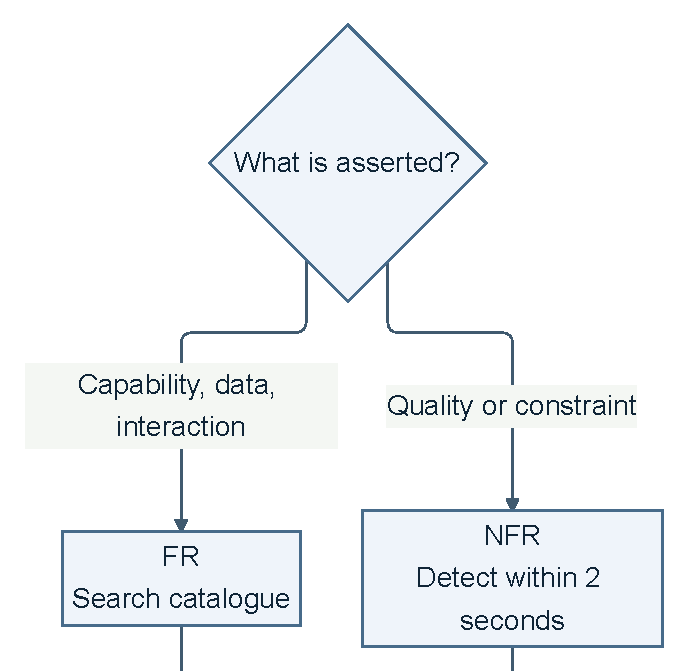
\includegraphics[width=202.86pt]{images/fig-003-compact-1.pdf}\end{minipage}\hfill
\begin{minipage}[t]{0.488\linewidth}\centering\scriptsize\textbf{2}\par\smallskip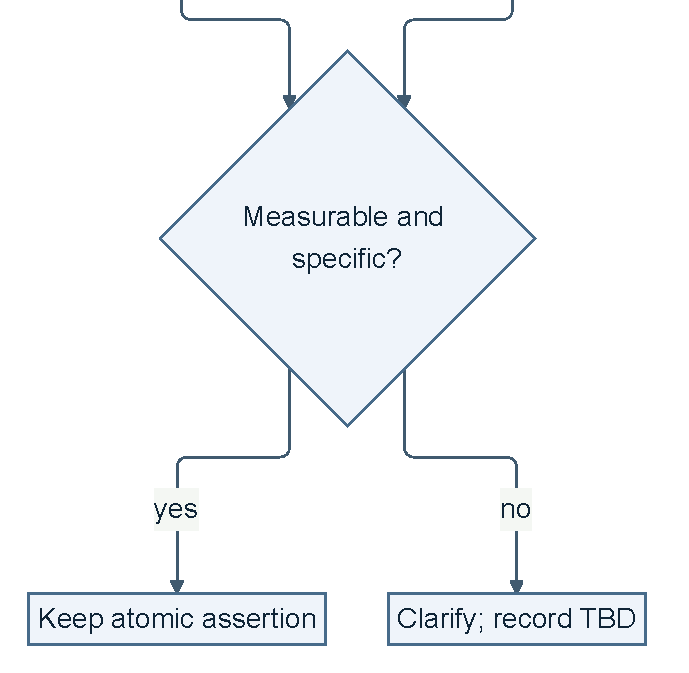
\includegraphics[width=202.86pt]{images/fig-003-compact-2.pdf}\end{minipage}
\captionof{figure}{classify a requirement --- follow numbered panels; crossing arrows continue.}\end{minipage}\par\smallskip

\begin{studycolumns}
\vspace{0pt}



\needspace{4\baselineskip}
\subsection*{2.1 Project mission statement}
\sectionlabel{h-21-project-mission-statement}
Two or three sentences that define:

\begin{enumerate}
\item \textbf{The problem} --- what will be done (scope and limits).
\item \textbf{The stakeholders} --- developers and users.
\item \textbf{The outcomes and benefits} --- plus a completion criterion.
\end{enumerate}


A mission statement may appear in the SRS product description (Writing SRS pp. 7--8).

\needspace{4\baselineskip}
\subsection*{2.2 Elicitation techniques (six --- memorise the list)}
\sectionlabel{h-22-elicitation-techniques-six--memorise-the-list}

\begin{referenceentries}
\textit{\textbf{Technique} / \textbf{Use when}}\par\smallskip
\noindent \textbf{\textbf{Interview}}: You need depth from one stakeholder; open questions\par
\noindent \textbf{\textbf{Observation}}: Users cannot articulate what they do ("watch the work")\par
\noindent \textbf{\textbf{Workshop}}: Many stakeholders must agree; resolve conflicts fast\par
\noindent \textbf{\textbf{Legacy product study}}: Replacing an existing system; inherit its quirks\par
\noindent \textbf{\textbf{Competitive product study}}: No access to users; derive features from rivals\par
\noindent \textbf{\textbf{Prototype}}: Requirements are visual/\allowbreak{}interaction-heavy; "a picture is worth a thousand words"\par
\end{referenceentries}
Two goals behind all six: \textbf{learn the problem domain} and \textbf{study user tasks}.

\textbf{Trap:} prototypes can elicit needs or validate them; state which purpose applies.
\end{studycolumns}

\Needspace{4\baselineskip}
\subsection*{2.3 Functional vs non-functional requirements}
\sectionlabel{h-23-functional-vs-non-functional-requirements}


{\fontsize{9}{11}\selectfont
\begin{longtable}{L{\dimexpr 0.17184\linewidth-4.12pt\relax}L{\dimexpr 0.40431\linewidth-9.70pt\relax}L{\dimexpr 0.42384\linewidth-10.17pt\relax}}
\toprule
\rowcolor{ice}\textbf{} & \textbf{\textbf{Functional}} & \textbf{\textbf{Non-functional}} \\
\midrule\endfirsthead
\toprule\rowcolor{ice}\textbf{} & \textbf{\textbf{Functional}} & \textbf{\textbf{Non-functional}} \\
\midrule\endhead
\multicolumn{3}{r}{\scriptsize Continued on next page}\\\endfoot
\bottomrule\endlastfoot
Definition & Interactions between the system and its environment; maps program inputs to program outputs & Properties the system must have, not directly related to functional behaviour \\
Answers & \emph{What must the system do?} & \emph{How well must it do it?} \\
Sub-kinds & System functionality \ensuremath{\cdot} Information to be processed \ensuremath{\cdot} Interface with other systems & Usability \ensuremath{\cdot} Reliability \ensuremath{\cdot} Performance \ensuremath{\cdot} Supportability (also security, availability, scalability, maintainability, portability) \\
Example & "The library member must be able to search the library catalog." & "When a book is placed on the checkout pad, the system must detect it within 2 seconds." \\
Example & "The system must display the temperature in degrees centigrade in the range \ensuremath{-}10 \textdegree{}C to +130 \textdegree{}C to one decimal place." & "Help messages must be displayed in the local language according to the user's locale." \\
Example & "The system must be able to control up to six robot arms simultaneously." & "After a system reboot, the full system functionality must be restored within 5 minutes." \\
\end{longtable}
}

\textbf{Classification drill (high-yield).} Decide which of these are FR vs NFR:




{\fontsize{9}{11}\selectfont
\begin{longtable}{L{\dimexpr 0.44456\linewidth-10.67pt\relax}L{\dimexpr 0.22664\linewidth-5.44pt\relax}L{\dimexpr 0.32880\linewidth-7.89pt\relax}}
\toprule
\rowcolor{ice}\textbf{Statement} & \textbf{Answer} & \textbf{Why} \\
\midrule\endfirsthead
\toprule\rowcolor{ice}\textbf{Statement} & \textbf{Answer} & \textbf{Why} \\
\midrule\endhead
\multicolumn{3}{r}{\scriptsize Continued on next page}\\\endfoot
\bottomrule\endlastfoot
The system must display the current time in 24-hour format & \textbf{FR} & Information to be processed \\
The database must be replaceable with any commercial product supporting standard SQL & \textbf{NFR} (supportability) & Portability/\allowbreak{}replaceability property \\
The system must verify membership with the University Account System before a loan & \textbf{FR} & Interface with another system \\
80\% of first-time users must enter a simple search query within 2 minutes & \textbf{NFR} (usability) & Measurable quality target \\
The system must log the event when the email server is unreachable & \textbf{FR} & Functionality (though see Section 3 --- may be an exception flow) \\
The system must be user-friendly & \textbf{NFR, but not verifiable as written} & Usability intent; needs a measurable criterion \\
\end{longtable}
}

\begin{studycolumns}
\vspace{0pt}


\begin{quote}\small\color{navy}
\textbf{Trap:} the "control up to six robot arms" example is \textbf{functional} (number of controllable devices is a capability), while "response within 2 seconds" is \textbf{performance/\allowbreak{}NFR}. Do not classify by the presence of a number --- classify by \textbf{what is being asserted}.

\end{quote}
\needspace{4\baselineskip}
\subsection*{2.4 Atomic, verifiable, traceable}
\sectionlabel{h-24-atomic-verifiable-traceable}
\textbf{Atomic} --- one testable assertion per numbered statement. Nest sub-requirements.


\begin{quote}\small\color{navy}
\emph{Original:} "When a computer is added, the tracking system requires the user to specify its type and allow the user to provide a description. Both these fields must be text of length > 0 and < 512."


\begin{ReferenceCode}
1.1   When a computer is added to the tracking system, the user must enter the computer type.
1.1.1 The computer type data must be text of at least one character and less than 512 characters.
1.2   When a computer is added to the tracking system, the user must enter a description.
1.2.1 The description of the computer must be text of at least one character and less than 512 characters.
\end{ReferenceCode}
\end{quote}
\textbf{Verifiable} --- sufficiently specific to be testable, with an oracle.


\begin{referenceentries}
\textit{\textbf{NO Not verifiable} / \textbf{YES Verifiable}}\par\smallskip
\noindent \textbf{NO Not verifiable:} The user interface must be user-friendly.\par
\noindent \textbf{YES Verifiable:} 80\% of first-time users must be able to enter a simple search query within 2 minutes of starting to use the system.\par\smallskip
\noindent \textbf{NO Not verifiable:} The system must control more than one drill press.\par
\noindent \textbf{YES Verifiable:} The system must control up to seven drill presses concurrently.\par\smallskip
\noindent \textbf{NO Not verifiable:} The company must not hire too-young or too-old people.\par
\noindent \textbf{YES Verifiable:} 0--15 and 55--99: do not hire; 16--17: part-time; 18--54: full-time.\par\smallskip
\end{referenceentries}
\textbf{Traceability} --- \emph{the ability to track requirements from their expression in the SRS to their realisation in design, documentation, source code, and their verification in reviews and tests; and to track dependencies among requirements, system functions and system components.}


\begin{quote}\small\color{navy}
\textbf{Trap:} traceability is \textbf{not} just "numbering requirements". Numbering is a prerequisite (modifiability); traceability is the \textbf{link} forwards (to design/\allowbreak{}code/\allowbreak{}test) and backwards (to source).

\end{quote}
\needspace{4\baselineskip}
\subsection*{2.5 Data dictionary (problem-domain glossary)}
\sectionlabel{h-25-data-dictionary-problem-domain-glossary}
The table below is the lecture's \textbf{illustrative university domain}, not a statement of NTU's academic calendar.

\begin{itemize}
\item Ensures \emph{consistent, unambiguous terminology} that all stakeholders agree on.
\item Defines \textbf{problem-domain} terms (Programme of Study, Course, Lecture, Tutorial, Class, Laboratory, Seminar) --- \textbf{not} implementation terms (table, foreign key, thread).
\end{itemize}

\begin{referenceentries}
\textit{\textbf{Term} / \textbf{Definition}}\par\smallskip
\noindent \textbf{Programme of Study}: A university programme a student enrols into. Three levels: undergraduate, master, PhD.\par
\noindent \textbf{Semester}: Four per academic year. Semesters 1 and 4 have 13 teaching weeks; semesters 2 and 3 have 5.\par
\noindent \textbf{Course}: A basic unit of teaching; compulsory or elective; must include lectures and tutorials; some have labs.\par
\noindent \textbf{Lecture}: Traditional class in lecture theatres; video recorded and published in the LMS.\par
\noindent \textbf{Tutorial}: Interactive, small-size class in technology-enhanced rooms; \textbf{not} video recorded.\par
\end{referenceentries}

\begin{quote}\small\color{navy}
\textbf{Trap:} the data dictionary is part of the SRS (Section 5 of the SRS contents). It is not a database schema and not a class diagram.

\end{quote}
\needspace{4\baselineskip}
\subsection*{2.6 Requirements validation}
\sectionlabel{h-26-requirements-validation}

\begin{referenceentries}
\textit{\textbf{Technique} / \textbf{What it checks}}\par\smallskip
\noindent \textbf{\textbf{Review} (walkthrough, inspection, critical review) with a checklist}: completeness, consistency, unambiguity, correctness\par
\noindent \textbf{\textbf{Prototype}}: Stakeholders: the system specified meets their needs/\allowbreak{}desires (\textbf{correct}) and requirements are \textbf{prioritised}. Development team: requirements and underlying assumptions are \textbf{properly understood}.\par
\end{referenceentries}

\begin{quote}\small\color{navy}
\textbf{Trap:} review \ensuremath{\neq} testing. Review is \textbf{static} (document inspection); testing is \textbf{dynamic} (execution). Both appear as "validation" in different lectures --- read the context.

\end{quote}
\needspace{4\baselineskip}
\subsection*{2.7 The iterative elicitation loop (memorise the steps)}
\sectionlabel{h-27-the-iterative-elicitation-loop-memorise-the-steps}
\textbf{Step 1 --- Project team alone.} Review the client's specification (and legacy/\allowbreak{}competitive products) to:

\begin{enumerate}
\item \textbf{Atomise} requirements.
\item Identify \textbf{actors}.
\item Identify main \textbf{use cases} (functional requirements).
\item Identify \textbf{non-functional} requirements.
\item Initiate the \textbf{data dictionary}.
\item Identify \textbf{uncertainties \ensuremath{\rightarrow} TBD} (To Be Determined). \emph{Never guess user requirements.}
\end{enumerate}
\textbf{Step 2 --- Project team meets client} (interview /\allowbreak{} observation /\allowbreak{} workshop). Agenda agreed up-front:

\begin{enumerate}
\item Present and walk through the initial requirements + data dictionary \ensuremath{\rightarrow} get agreement.
\item Clarify the TBD issues.
\item Discuss new requirements the client raises.
\end{enumerate}
Repeat 1--2 \textbf{until} all uncertainties and ambiguities in functional, non-functional requirements and data-dictionary terms are agreed with the client. A prototype may be produced to show intended functionality. \textbf{Minimise the number of meetings by making meetings productive.}


\begin{quote}\small\color{navy}
\textbf{Trap:} "Do not guess the user requirements" is an explicit lecture instruction --- the correct answer to a missing requirement is \textbf{TBD + ask the client}, not "assume a sensible default".

\end{quote}
\end{studycolumns}
